\documentclass[a4paper]{article}

\addtolength{\hoffset}{-2.25cm}
\addtolength{\textwidth}{4.5cm}
\addtolength{\voffset}{-3.25cm}
\addtolength{\textheight}{5cm}
\setlength{\parskip}{0pt}
\setlength{\parindent}{0in}

%----------------------------------------------------------------------------------------
%	PACKAGES AND OTHER DOCUMENT CONFIGURATIONS
%----------------------------------------------------------------------------------------

\usepackage{blindtext} % Package to generate dummy text
\usepackage{charter} % Use the Charter font
\usepackage[utf8]{inputenc} % Use UTF-8 encoding
\usepackage{microtype} % Slightly tweak font spacing for aesthetics
\usepackage[english]{babel} % Language hyphenation and typographical rules
\usepackage{amsthm, amsmath, amssymb} % Mathematical typesetting
\usepackage{float} % Improved interface for floating objects
\usepackage[final, colorlinks = true,
            linkcolor = black,
            citecolor = black]{hyperref} % For hyperlinks in the PDF
\usepackage{graphicx, multicol} % Enhanced support for graphics
\usepackage{xcolor} % Driver-independent color extensions
\usepackage{marvosym, wasysym} % More symbols
\usepackage{rotating} % Rotation tools
\usepackage{censor} % Facilities for controlling restricted text
\usepackage{listings} % Environment for non-formatted code, !uses style file!
\usepackage{pseudocode} % Environment for specifying algorithms in a natural way
 % Environment for f-structures, !uses style file!
\usepackage{booktabs} % Enhances quality of tables
\usepackage{tikz-qtree} % Easy tree drawing tool
 % Configuration for b-trees and b+-trees, !uses style file!
\usepackage[backend=bibtex,style=numeric,
            sorting=nyt]{biblatex} % Complete reimplementation of bibliographic facilities
\addbibresource{b.bib}
\usepackage{csquotes} % Context sensitive quotation facilities
\usepackage[yyyymmdd]{datetime} % Uses YEAR-MONTH-DAY format for dates
\renewcommand{\dateseparator}{-} % Sets dateseparator to '-'
\usepackage{fancyhdr} % Headers and footers
\pagestyle{fancy} % All pages have headers and footers
\fancyhead{}\renewcommand{\headrulewidth}{0pt} % Blank out the default header
\fancyfoot[L]{} % Custom footer text
\fancyfoot[C]{} % Custom footer text
\fancyfoot[R]{\thepage} % Custom footer text
\newcommand{\note}[1]{\marginpar{\scriptsize \textcolor{red}{#1}}} % Enables comments in red on margin
\usepackage{mathtools}
\usepackage{amsmath}
\DeclarePairedDelimiter\abs{\lvert}{\rvert}%
\usepackage{cancel}
\usepackage{minted}
\usepackage{float}
\usepackage{caption}
\usepackage{subcaption}
%-------------------------------

%----------------------------------------------------------------------------------------
\nocite{*}
%-------------------------------
%	ENVIRONMENT SECTION
%-------------------------------
\pagestyle{fancy}
\usepackage{mdframed}

\usepackage[sfdefault]{FiraSans} %% option 'sfdefault' activates Fira Sans as the default text font
\usepackage[T1]{fontenc}
\renewcommand*\oldstylenums[1]{{\firaoldstyle #1}}


% remove numbering from sections
\usepackage{titlesec}
\titleformat{\section}{\normalfont\Large\bfseries}{}{0pt}{}


% Reference


%-------------------------------------------------------------------------------------------
%	CUSTOM COMMANDS
%-------------------------------
\newcommand{\gaussian}{\frac{1}{\sigma\sqrt{2\pi}}\exp\left(- \frac{(x-\mu)^2}{2\sigma^2}\right)}
\newcommand{\R}{\mathbb R}
\newcommand{\norm}[1]{\lVert #1 \rVert}

\def\inline{\lstinline[basicstyle=\ttfamily,keywordstyle={}]}


\newcommand{\ps}{x^+}
\newcommand{\ns}{x^-}


\begin{document}


%-------------------------------
%	TITLE SECTION
%-------------------------------

\fancyhead[C]{}
\hrule \medskip % Upper rule
\begin{minipage}{0.295\textwidth}
  \raggedright
  \footnotesize
  Francisco Javier Sáez Maldonado \hfill\\
  franciscojavier.saez@estudiante.uam.es
  \hfill\\
\end{minipage}
\begin{minipage}{0.4\textwidth}
  \centering
  \large
  Speaker Recognition\\
  \normalsize
  Deep Learning for Audio Signals\\
\end{minipage}
\begin{minipage}{0.295\textwidth}
  \raggedleft
  \today\hfill\\
\end{minipage}
\medskip\hrule

%-------------------------------
%	CONTENTS
%-------------------------------

\tableofcontents

\section*{Introduction}

Speaker recognition is the task of identifying a person from his/her voice. In this lab report, we will examine a speaker recognition system that will use \emph{x-vectors} embeddings to classify the speakers. The system has been developed to solve the \href{https://www.robots.ox.ac.uk/~vgg/data/voxceleb/competition2020.html}{VoxCeleb} challenge.\\

The system \emph{extracts} the fixed-size embeddings trying to include in these representations as much discriminative information as possible for the speaker recognition task. A few architectures of neural networks can be used with this purpose, as well as different loss functions.\\

The code that I used to test the model, which was provided by \href{http://audias.ii.uam.es/staff/}{Alicia Lozano}, can be found in this \href{https://drive.google.com/file/d/1aWhFcbRUTJ0sOtYNPvLjHencfINu8SFz/view?usp=sharing}{link}.

\section{Examining the code}

In this section, we will examine the provided code in order to find the most relevant parts of it. Let us begin by examining the \inline{trainSpeakerNet.py} file, since it is the main script. The code is properly commented so identifying the different parts is quite simple.\\

\textbf{Questions.}\\

\begin{itemize}
  \item \emph{Which line of the code trains the model?}\\

        We found \inline{line 169}:
        \begin{minted}{Python}
    loss, traineer = s.train_network(loader=trainLoader);
  \end{minted}
        which trains the code. The variable \inline{s} was previously initialized as \inline{s = SpeakerNet(**vars(args));}, creating an instance of the SpeakerNet defined model class. This class has the called \inline{train_network} function, which performs (vaguely explained) a classic forward pass with loss computation and returns the average loss and the \inline{train eer}.

  \item \emph{Which command loads a pre-trained model?}\\

        Having a look from lines \(112-121\), we find that in lines \(116\) and \(120\), the function \inline{s.loadParameters(args)} is called. This function loads the pretrained model from a specific file. As we can see in the code, a distinction is made in our case, being able to load the model from the \inline{save_path} or from the argument \inline{args.initial_model}.
  \item \emph{Which line evaluates the performance of the neural network?}\\

        A few lines below the training line, in line \inline{176} we find:
        \begin{minted}[]{Python}
    sc, lab, _ = s.evaluateFromList(args.test_list, print_interval=100,
                                    test_path=args.test_path, eval_frames=args.eval_frames)
  \end{minted}
        which evaluates the model in the \inline{test_list}. In this function, all the features for each of the test file audios (\emph{.wav}) files are extracted and then the scores are computed using \inline{pairwise_distance}.

  \item \emph{Which variable contains the scores of the trials list? In which file are those scores saved?}\\

        Firstly, we find in line \inline{176} that the scores of the trials are stored in the variable \inline{sc}. Then, in line \inline{177} we observe that the scores are thresholded and stored in the variable \inline{result}. Then, they are saved in the \inline{scorefile} file. This is a variable that, in line \(150\) opened a file called \inline{result_save_path/scores.txt}, where \inline{result_save_path} came as an argument from the execution of the script.

  \item \emph{Which variable controls the number of epochs(iterations) that the model is trained?}\\

        We find in line \(198\) and \(201\) that the variable \inline{it} is modified and checks the \inline{max_epoch} indicated as an argument. Then, is the variable \inline{max_epoch} the one that controls the number of epochs that the model is trained.

  \item \emph{Which parameter determines the loss function?}\\

        We find that in line \(29\) the argument \inline{--trainfunc} with description \emph{'Loss function'} is declared. Then, it is passed to the model class in the creation of the instance of the model (passing all the arguments at the same time).

  \item \emph{What is the purpose of the parameter \inline{test_interval}?}\\

        Having a look at the description of the parameters, in \inline{line 27} we read that this parameter controls how many train epochs we make before every evaluation. For instance, if \(test\_interval = 10\), then every \(10\) training epoch we perform an evaluation on the \inline{test_list} (\inline{line 176}) and save the results.

  \item \emph{Which argument has to be modified in order to change the architecture of the model?}\\


        The architecture of the model is defined in the argument \inline{--model}. As we can see, in the folder \inline{models}, there are a few implementations of \inline{ResNet} and \inline{VGG} that could be used to change the architecture of the model.

  \item \emph{What is the purpose of the parameter \inline{nClasses}? How would you obtain this value from the dataset? Write the command that you would use.}\\

        The parameter \inline{nClasses} controls the number of speakers that are used in the softmax layer. Let us explain how we would obtain this from the dataset. As we are explained in the provided jupyter notebook, the training data is stored in the folder \inline{data/voxceleb2}. Inside this folder, we find a large number of subfolders, each one containing the audios from a different speaker, which \textbf{represents a class} in our problem. So, to obtain the parameter \inline{nClasses}, we would have to count the number of folders stored in the directory \inline{data/voxceleb2}. We can do this in linux by using a \inline{pipe}, listing the folders in the directory and then counting the number of lines (using the linux command \inline{wc -l}). The execution provides the following result:

        \begin{minted}{bash}
           !ls data/voxceleb2/ | wc -l

           4953
        \end{minted}


        It has to be remarked that the validation set does not have the same number of unique classes. When we execute this same command in the folder \inline{data/voxceleb1}, we obtain that there are only \(40\) classes.

\end{itemize}


\section{Evaluating pretrained models}

We are given two pretrained models using the \emph{VoxCeleb2} dataset (the dev partition). In this section, we evaluate the models and compare the results. To evaluate the models, we have to execute the previous script, using the argument \inline{--eval} as well as the dataset path, the model type and some extra parameters. We show the execution output (removing the \inline{warning} lines).\\

\textbf{First Model:}\\
\begin{minted}{bash}
!python ./trainSpeakerNet.py --eval --model ResNetSE34L --log_input True \
          --trainfunc angleproto --save_path exps/test_lite --eval_frames 400 \
          --test_list lists/veri_test.txt \
          --initial_model pretrained_models/baseline_lite_ap.model


Embedding size is 512, encoder SAP.
Initialised AngleProto
Initialised Adam optimizer
Initialised step LR scheduler
Model has 1437080 parameters
Model pretrained_models/baseline_lite_ap.model loaded!
Reading 4700 of 4715: 28.75 Hz, embedding size 512
Computing 37700 of 37720: 1776.69 Hz

EER 2.1792
\end{minted}

\textbf{Second Model:}\\
\begin{minted}{bash}
!python ./trainSpeakerNet.py --eval --model ResNetSE34V2 --log_input True \
  --encoder_type ASP --n_mels 64 --trainfunc softmaxproto \
  --save_path exps/test_v2 --eval_frames 400 --test_list lists/veri_test.txt \
  --initial_model pretrained_models/baseline_v2_ap.model

Embedding size is 512, encoder ASP.
Initialised Softmax Loss
Initialised AngleProto
Initialised SoftmaxPrototypical Loss
Initialised Adam optimizer
Initialised step LR scheduler
Model has 11103416 parameters
Model pretrained_models/baseline_v2_ap.model loaded!
Reading 4700 of 4715: 4.19 Hz, embedding size 512
Computing 37700 of 37720: 1766.00 Hz

EER 1.1771
\end{minted}

\textbf{Questions.}\\

\begin{itemize}
  \item \emph{How does each of the previous model perform?}\\

        We obtain the following results:
        \begin{itemize}
          \item Model 1 EER: \(2.1792\).
          \item Model 2 EER: \(1.1771\).
        \end{itemize}

  Further explanation on these results will be provided in the following questions.

  \item \emph{Which one is the best and why?}\\

        As we will explain in the following question, the lower the EER is, the better the model is. This implies that, in our case, the second model is better than the first one.

  \item \emph{What is the EER and how can we interpret it?}\\

        EER stands for \textbf{Equal Error Rate}. To understand this concept, we assume that the concepts of \emph{TP, TN, FP, and FN} are known. Using these concepts and considering \(N\) as the total number of examples, we can define the \textbf{False Rejection Rate (FFR)} and \textbf{False Aceptation Rate (FAR)} as the ratios:
        \[
        FFR = \frac{FN}{N}, \quad FAR = \frac{FP}{N}.
        \]

        For each of these two metrics, we have to choose a \emph{threshold} that we would like our model to fulfill, using the number of \emph{allowed False Positives and False Negatives}. The \textbf{Dectection Error Tradeoff (DET)} curve represents this tradeoff trying to decrease both FAR and FFR. We can see an example of DET curve in Figure \ref{fig:DET}.

        \begin{figure}
          \centering
          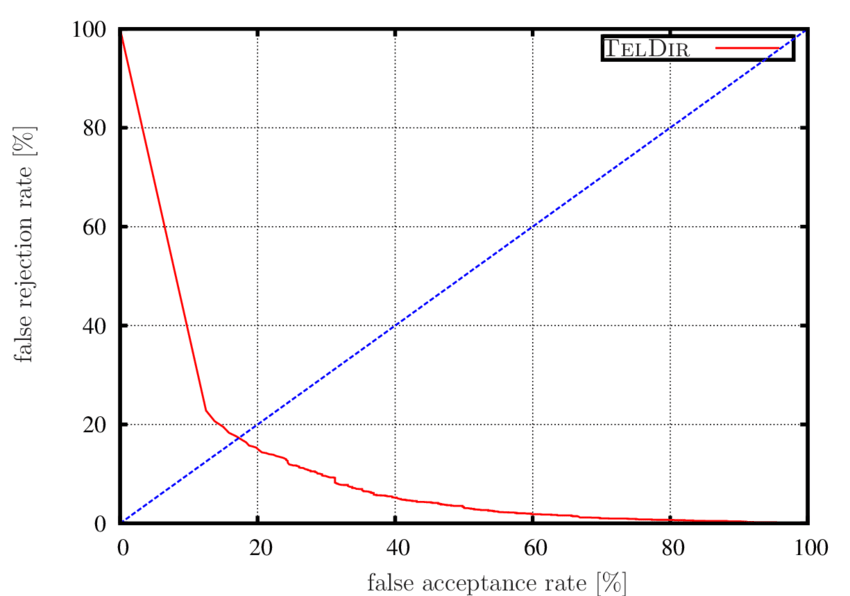
\includegraphics[scale=0.4]{Figures/DET}
          \caption{Example of DET curve.}
          \label{fig:DET}
        \end{figure}

        With all these concept, we can define the EER as the point of the DET curve where \(FAR = FRR\), that is, the point where our model rejects the same amount of positive examples than the number of negative samples that it accepts.

        At this point, we get to understand why a lower EER is better, since if the EER is lower it means that both our FAR and FFR (which are \emph{negative} quantities) are low.
  \item \emph{What are the differences between the models?}\\



\end{itemize}


\section{Training a model}

In this section, we are given a few specifications for a model and we are asked to train a model using the provided specifications. In particular, the specifications are:

\begin{itemize}
  \item The \textbf{encoder} must be a \inline{ResNetSE34L} with \inline{SAP} (which does not increase the out dimension of the linear layer of the model).
  \item Loss function \textbf{amsoftmax}
  \item \inline{Scale = 30}
  \item \inline{margin = 0.3}
  \item Number of speaker equal to the number of classes (we found before that the number is \(4953\)).
        \item Fix a number of epochs. In our case, we tested a few different numbers, fixing the final number to \(100\) epoch (leading to a training that lasts more than one hour).
\end{itemize}


\section{Extra: Training a model of our choice}
In this last section, we are asked to train a model of our choice, choosing an \textbf{encoder} and

The choice I made was to select

\subsection{Intuitions on triplet losses}

\emph{x-vectors} are representations of the audio signals we are dealing with. Ideally, we would like to obtain intermediate representations in our encoder that, given an input data $x$, preserve the distance between similar data points close and also makes de distance between different datapoints far on the embedding space \cite{Sohn2016ImprovedDM}.

Let us set the notation that we will use first. We will consider sets of triplets $(x,\ps,\ns)$ where:
\begin{itemize}
\item The element $x$ is an anchor point,
\item The element $\ps$ is a positive instance,
\item The element $\ns$ is a negative instance.
\end{itemize}

The main idea is to learn a representation of $x$, say $g(x)$, such that the distance of the representation of the input is closer in distance to the representation of the positive sample $\ps$ than the representation of the negative sample $\ns$. Using the norm, we can formally express that as follows:
$$
\norm{g(x) - g(\ps)}_2 \leq \norm{g(x) - g(\ns)}_2,
$$
for each triplet in the set.\\

The loss function that we will use will use this inequality, adding a last term, which we will motivate now: Support-vector machines (SVMs) are supervised learning models used for classification or regression problems. They are one of the most robust prediction methods. They search for a hyperplane $h$ in high or infinite dimensional space that separates the data as much as possible, making use of \emph{support vectors}, the datapoints that are closest to the hyperplane. If the data is linearly separable, we can select two hyperplanes $h_1,h_2$ that are parallel to $h$ and making the distance from them to $h$ as large as possible. That region is called the \emph{margin}.\\

Coming back to our triplets problem, we also want to introduce a margin between the distances of the elements of the triplets, in order to separate positive examples from negative examples as much as possible. This way, we introduce a \emph{margin} term $\alpha$, rewriting our last equation as follows:
\[
\norm{g(x) - g(\ps)}_2 + \alpha < \norm{g(x) - g(\ns)}_2.
\]
Using this inequality, we can define a loss function for each triplet in the set:
\begin{equation}\label{triplet:single:loss}
\ell^\alpha (x,\ps,\ns) =  \norm{g(x) - g(\ps)}_2^2 - \norm{g(x) - g(\ns)}_2^2 + \alpha.
\end{equation}
This loss has been defined for a single triplet. This is the loss function that we have defined in the file \inline{loss/triplet.py}.


\printbibliography

\end{document}
